\section{Resultados e discussão}\label{sec:resultados}

Todos os números desta seção são gerados pelos scripts de análise a partir dos
arquivos brutos e inseridos no texto por macros; nenhum valor foi digitado à
mão. Foram realizadas \NExecTotal{} execuções de simulação, com
\NExecErros{} falhas de execução, totalizando \CPUhoras{} horas de
processamento.

% provisório: 06a-plataforma


\subsection{Comparação principal (E1)}\label{sec:e1}

A Tabela~\ref{tab:e1} e a Figura~\ref{fig:e1} resumem o desempenho das cinco
políticas nas três escalas. As comparações pareadas com A estão nas
Tabelas~\ref{tab:e1km} e~\ref{tab:e1ov}.

\begin{table}[ht]
\centering
\caption{E1 -- médias por política e escala (30 sementes; IC 95\% \emph{bootstrap} entre colchetes). ``Espera'': tempo médio entre o contêiner atingir 80\% e ser coletado.}
\label{tab:e1}
\scriptsize
\setlength{\tabcolsep}{3.5pt}
\resizebox{\textwidth}{!}{\begin{tabular}{@{}clcccccc@{}}
\toprule
$N$ & Pol. & km/dia [IC 95\%] & Transb. \% [IC 95\%] & Ocup. coleta (\%) & Coletas $<$50\% (\%) & Visitas/dia & Espera (h) \\
\midrule
20 & \polA{} & 59,5 [56,1; 63,0] & 1,37 [1,08; 1,74] & 64 & 24,5 & 9,1 & 13,1 \\
 & \polB{} & 50,1 [47,6; 52,6] & 5,35 [4,72; 5,99] & 92 & 0,0 & 6,1 & 14,0 \\
 & \polBOR{} & 49,8 [47,4; 52,2] & 5,31 [4,66; 5,96] & 92 & 0,0 & 6,1 & 14,0 \\
 & \polC{} & 47,8 [45,2; 50,4] & 4,24 [3,67; 4,87] & 85 & 0,4 & 6,7 & 13,3 \\
 & \polD{} & 55,8 [52,9; 58,7] & 1,10 [0,86; 1,42] & 68 & 16,2 & 8,7 & 9,3 \\
\midrule
100 & \polA{} & 120,0 [118,2; 121,9] & 1,28 [1,20; 1,36] & 63 & 26,0 & 45,9 & 12,9 \\
 & \polB{} & 121,7 [119,5; 124,1] & 5,79 [5,62; 5,95] & 92 & 0,0 & 30,1 & 14,4 \\
 & \polBOR{} & 100,1 [98,4; 101,8] & 5,77 [5,58; 5,96] & 92 & 0,0 & 30,2 & 14,3 \\
 & \polC{} & 96,2 [94,4; 98,1] & 3,61 [3,48; 3,74] & 81 & 0,7 & 35,1 & 12,8 \\
 & \polD{} & 112,2 [110,5; 114,1] & 0,92 [0,85; 1,00] & 66 & 17,3 & 44,1 & 8,9 \\
\midrule
500 & \polA{} & 350,8 [348,0; 353,4] & 1,20 [1,16; 1,24] & 63 & 25,3 & 230,2 & 13,3 \\
 & \polB{} & 364,7 [361,2; 368,0] & 5,31 [5,20; 5,42] & 91 & 0,0 & 153,1 & 14,0 \\
 & \polBOR{} & 304,3 [302,0; 306,6] & 5,27 [5,16; 5,37] & 91 & 0,0 & 153,2 & 14,0 \\
 & \polC{} & 307,2 [304,3; 310,1] & 2,24 [2,17; 2,31] & 75 & 1,3 & 193,7 & 11,5 \\
 & \polD{} & 332,3 [330,2; 334,4] & 0,63 [0,60; 0,67] & 63 & 21,7 & 234,4 & 8,8 \\
\bottomrule
\end{tabular}
}
\end{table}

\begin{figure}[ht]
  \centering
  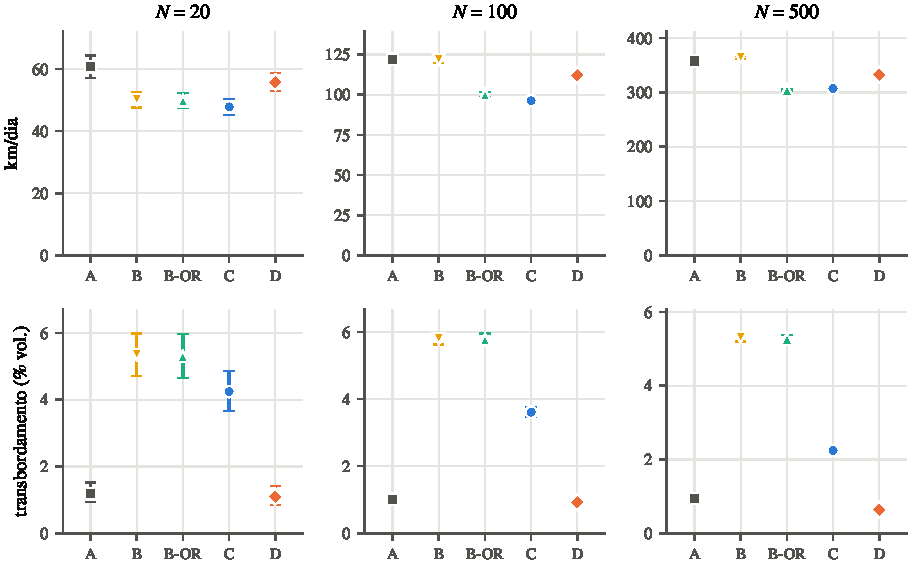
\includegraphics[width=\textwidth]{figures/fig_e1.pdf}
  \caption{E1 -- distância diária e transbordamento por política e escala (média e IC 95\%, 30 sementes).}
  \label{fig:e1}
\end{figure}

\paragraph{Quando coletar (QP1).}
Com os dados de nível, as políticas B e C coletam contêineres mais cheios:
em $N = 100$, a ocupação verdadeira média na coleta foi de \FillNCemB\% (B) e
\FillNCemC\% (C), contra \FillNCemA\% na coleta periódica, e as coletas com
ocupação abaixo de 50\% caíram de \BelowNCemA\% (A) para \BelowNCemB\% (B) e
\BelowNCemC\% (C). A distribuição completa (Figura~\ref{fig:hist}) mostra que A
espalha as coletas por toda a faixa de ocupação, enquanto B as concentra
acima de 75\%. A política preditiva ocupa uma posição intermediária
(\FillNCemD\% de ocupação média; \BelowNCemD\% de coletas abaixo de 50\%):
ela antecipa visitas a contêineres que provavelmente transbordariam antes da
próxima oportunidade e, ao fazê-lo, aceita coletá-los mais vazios. Coletar
mais cheio, portanto, não é sinônimo de coletar melhor: as políticas que mais
elevam a ocupação na coleta são também as que mais deixam contêineres
transbordar.

\begin{figure}[ht]
  \centering
  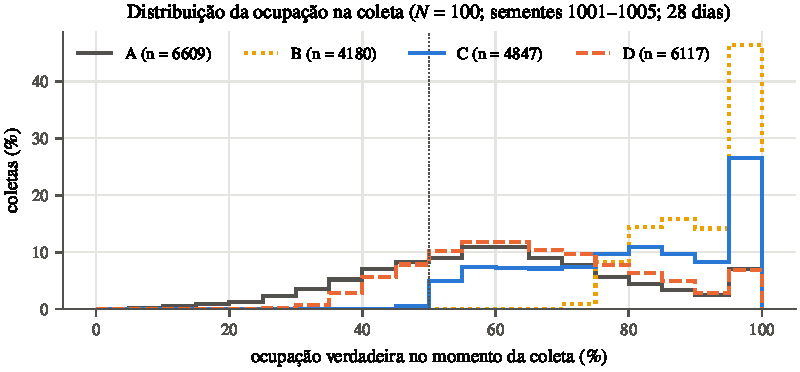
\includegraphics[width=\textwidth]{figures/fig_hist_coleta.pdf}
  \caption{Distribuição da ocupação verdadeira no momento da coleta ($N=100$; cinco sementes; 28 dias avaliados).}
  \label{fig:hist}
\end{figure}

\paragraph{Diferenças operacionais (QP2).}
Os resultados confirmam parcialmente as hipóteses pré-especificadas.
\emph{H2a} se confirma: C percorreu menos que A em todas as escalas, com
redução de \RelNVinteCvsAKm\%, \RelNCemCvsAKm\% e \RelNQuinhentosCvsAKm\% para
20, 100 e 500 contêineres ($p_{\mathrm{Holm}}$ \PNCemCvsAKm{} em $N = 100$;
$r_{rb} = -1$, isto é, menor distância em todas as 30 sementes). Mas essa
economia veio acompanhada de transbordamento maior: \OvNCemC\% do volume
gerado em C contra \OvNCemA\% em A ($N = 100$), uma diferença de
\DifNCemCvsAOv{} pontos percentuais (IC 95\%: \LoNCemCvsAOv{} a
\HiNCemCvsAOv). \emph{H2b} se confirma com folga: B transbordou
\OvNCemB\% do volume em $N = 100$, cerca de quatro vezes o valor de A, e só
visita contêineres que já estão perto do limite. O roteirizador também pesa:
com o vizinho mais próximo e 2-opt, B percorreu \RelNCemBvsAKm\% e
\RelNQuinhentosBvsAKm\% a mais que A em $N = 100$ e $N = 500$; com o OR-Tools
(B-OR), a mesma seleção percorreu \RelNCemBORvsAKm\% e
\RelNQuinhentosBORvsAKm\% em relação a A. Isso mostra que parte do ganho
atribuído à ``coleta inteligente'' em comparações informais pode vir apenas da
qualidade do roteirizador.

\emph{H2c} também se confirma: D transbordou menos que C em todas as escalas
(\OvNCemD\% contra \OvNCemC\% em $N = 100$; $p_{\mathrm{Holm}}$
\PNCemDvsCOv) e percorreu mais (\RelNCemDvsCKm\%). O resultado mais
relevante para a questão prática, porém, é a comparação com a linha de base:
D percorreu \RelNCemDvsAKm\% e \RelNQuinhentosDvsAKm\% em relação a A, em
$N = 100$ e $N = 500$, e ao mesmo tempo transbordou menos
(\RelNCemDvsAOv\% e \RelNQuinhentosDvsAOv\%; $p_{\mathrm{Holm}}$
\PNCemDvsAOv{} e \PNQuinhentosDvsAOv). Em $N = 20$, a redução de distância de
D (\RelNVinteDvsAKm\%) foi significativa, mas a de transbordamento
(\RelNVinteDvsAOv\%) não foi ($p_{\mathrm{Holm}} = $~\PNVinteDvsAOv). Com
poucos contêineres espalhados pela cidade, cada visita exige deslocamentos
longos, e a escolha de quais pontos visitar tem pouco efeito sobre a
distância total.

\begin{table}[ht]
\centering
\caption{E1 -- comparações pareadas de km/dia (alternativa $-$ referência; 30 pares; $r_{rb}$: correlação bisserial de postos; $p$ ajustado por Holm na família E1/km).}
\label{tab:e1km}
\scriptsize
\resizebox{\textwidth}{!}{\begin{tabular}{@{}llrcrrr@{}}
\toprule
Escala & Comparação & Dif. média & IC 95\% & Dif. (\%) & $r_{rb}$ & $p$ (Holm) \\
\midrule
$N=20$ & \polB{} $-$ \polA{} & $-$9,40 & [$-$10,80; $-$8,11] & $-$15,8 & $-$1,00 & $<$0,001 \\
$N=20$ & \polBOR{} $-$ \polA{} & $-$9,74 & [$-$11,20; $-$8,35] & $-$16,4 & $-$1,00 & $<$0,001 \\
$N=20$ & \polC{} $-$ \polA{} & $-$11,72 & [$-$13,11; $-$10,33] & $-$19,7 & $-$1,00 & $<$0,001 \\
$N=20$ & \polD{} $-$ \polA{} & $-$3,71 & [$-$4,70; $-$2,73] & $-$6,2 & $-$0,91 & $<$0,001 \\
$N=20$ & \polD{} $-$ \polC{} & 8,01 & [7,17; 8,84] & 16,8 & 1,00 & $<$0,001 \\
$N=20$ & \polC{} $-$ \polBOR{} & $-$1,98 & [$-$2,53; $-$1,44] & $-$4,0 & $-$0,94 & $<$0,001 \\
$N=20$ & \polBOR{} $-$ \polB{} & $-$0,33 & [$-$0,58; $-$0,11] & $-$0,7 & $-$0,57 & 0,014 \\
$N=100$ & \polB{} $-$ \polA{} & 1,75 & [0,17; 3,34] & 1,5 & 0,49 & 0,017 \\
$N=100$ & \polBOR{} $-$ \polA{} & $-$19,94 & [$-$20,91; $-$18,99] & $-$16,6 & $-$1,00 & $<$0,001 \\
$N=100$ & \polC{} $-$ \polA{} & $-$23,78 & [$-$24,77; $-$22,86] & $-$19,8 & $-$1,00 & $<$0,001 \\
$N=100$ & \polD{} $-$ \polA{} & $-$7,76 & [$-$8,60; $-$6,94] & $-$6,5 & $-$1,00 & $<$0,001 \\
$N=100$ & \polD{} $-$ \polC{} & 16,01 & [15,26; 16,73] & 16,6 & 1,00 & $<$0,001 \\
$N=100$ & \polC{} $-$ \polBOR{} & $-$3,84 & [$-$4,71; $-$3,03] & $-$3,8 & $-$1,00 & $<$0,001 \\
$N=100$ & \polBOR{} $-$ \polB{} & $-$21,70 & [$-$22,88; $-$20,58] & $-$17,8 & $-$1,00 & $<$0,001 \\
$N=500$ & \polB{} $-$ \polA{} & 13,84 & [11,33; 16,48] & 3,9 & 1,00 & $<$0,001 \\
$N=500$ & \polBOR{} $-$ \polA{} & $-$46,56 & [$-$48,14; $-$45,01] & $-$13,3 & $-$1,00 & $<$0,001 \\
$N=500$ & \polC{} $-$ \polA{} & $-$43,61 & [$-$44,97; $-$42,29] & $-$12,4 & $-$1,00 & $<$0,001 \\
$N=500$ & \polD{} $-$ \polA{} & $-$18,49 & [$-$19,91; $-$17,02] & $-$5,3 & $-$1,00 & $<$0,001 \\
$N=500$ & \polD{} $-$ \polC{} & 25,12 & [23,43; 26,76] & 8,2 & 1,00 & $<$0,001 \\
$N=500$ & \polC{} $-$ \polBOR{} & 2,95 & [1,20; 4,76] & 1,0 & 0,58 & 0,013 \\
$N=500$ & \polBOR{} $-$ \polB{} & $-$60,40 & [$-$63,16; $-$57,69] & $-$16,6 & $-$1,00 & $<$0,001 \\
\bottomrule
\end{tabular}
}
\end{table}

\begin{table}[ht]
\centering
\caption{E1 -- comparações pareadas de transbordamento (pontos percentuais do volume gerado; mesma estrutura da Tabela~\ref{tab:e1km}).}
\label{tab:e1ov}
\scriptsize
\resizebox{\textwidth}{!}{\begin{tabular}{@{}llrcrrr@{}}
\toprule
Escala & Comparação & Dif. média & IC 95\% & Dif. (\%) & $r_{rb}$ & $p$ (Holm) \\
\midrule
$N=20$ & \polB{} $-$ \polA{} & 3,98 & [3,44; 4,55] & 289,6 & 1,00 & $<$0,001 \\
$N=20$ & \polBOR{} $-$ \polA{} & 3,93 & [3,38; 4,56] & 286,6 & 1,00 & $<$0,001 \\
$N=20$ & \polC{} $-$ \polA{} & 2,87 & [2,38; 3,44] & 209,0 & 1,00 & $<$0,001 \\
$N=20$ & \polD{} $-$ \polA{} & $-$0,28 & [$-$0,49; $-$0,07] & $-$20,1 & $-$0,49 & 0,070 \\
$N=20$ & \polD{} $-$ \polC{} & $-$3,15 & [$-$3,66; $-$2,67] & $-$74,2 & $-$1,00 & $<$0,001 \\
$N=20$ & \polC{} $-$ \polBOR{} & $-$1,06 & [$-$1,32; $-$0,82] & $-$20,1 & $-$0,97 & $<$0,001 \\
$N=20$ & \polBOR{} $-$ \polB{} & $-$0,04 & [$-$0,12; 0,03] & $-$0,8 & $-$0,19 & 0,762 \\
$N=100$ & \polB{} $-$ \polA{} & 4,51 & [4,35; 4,66] & 353,7 & 1,00 & $<$0,001 \\
$N=100$ & \polBOR{} $-$ \polA{} & 4,49 & [4,32; 4,66] & 352,4 & 1,00 & $<$0,001 \\
$N=100$ & \polC{} $-$ \polA{} & 2,34 & [2,20; 2,47] & 183,2 & 1,00 & $<$0,001 \\
$N=100$ & \polD{} $-$ \polA{} & $-$0,35 & [$-$0,43; $-$0,26] & $-$27,5 & $-$0,95 & $<$0,001 \\
$N=100$ & \polD{} $-$ \polC{} & $-$2,69 & [$-$2,80; $-$2,58] & $-$74,4 & $-$1,00 & $<$0,001 \\
$N=100$ & \polC{} $-$ \polBOR{} & $-$2,16 & [$-$2,28; $-$2,04] & $-$37,4 & $-$1,00 & $<$0,001 \\
$N=100$ & \polBOR{} $-$ \polB{} & $-$0,02 & [$-$0,09; 0,06] & $-$0,3 & $-$0,09 & 0,762 \\
$N=500$ & \polB{} $-$ \polA{} & 4,11 & [4,00; 4,22] & 343,7 & 1,00 & $<$0,001 \\
$N=500$ & \polBOR{} $-$ \polA{} & 4,07 & [3,96; 4,18] & 340,3 & 1,00 & $<$0,001 \\
$N=500$ & \polC{} $-$ \polA{} & 1,04 & [0,98; 1,11] & 87,2 & 1,00 & $<$0,001 \\
$N=500$ & \polD{} $-$ \polA{} & $-$0,56 & [$-$0,60; $-$0,52] & $-$47,1 & $-$1,00 & $<$0,001 \\
$N=500$ & \polD{} $-$ \polC{} & $-$1,61 & [$-$1,65; $-$1,56] & $-$71,8 & $-$1,00 & $<$0,001 \\
$N=500$ & \polC{} $-$ \polBOR{} & $-$3,03 & [$-$3,09; $-$2,96] & $-$57,5 & $-$1,00 & $<$0,001 \\
$N=500$ & \polBOR{} $-$ \polB{} & $-$0,04 & [$-$0,08; 0,00] & $-$0,8 & $-$0,34 & 0,315 \\
\bottomrule
\end{tabular}
}
\end{table}

\subsection{Mesmo nível de serviço: fronteiras distância $\times$ transbordamento (E2)}\label{sec:e2}

As comparações do E1 dependem dos parâmetros padrão de cada política: um
limiar de 75\% em C é uma escolha, e não uma propriedade da política. O E2
varia esses parâmetros e traça, para cada política, a curva de distância
necessária para cada nível de transbordamento (Figura~\ref{fig:e2}).

\begin{figure}[ht]
  \centering
  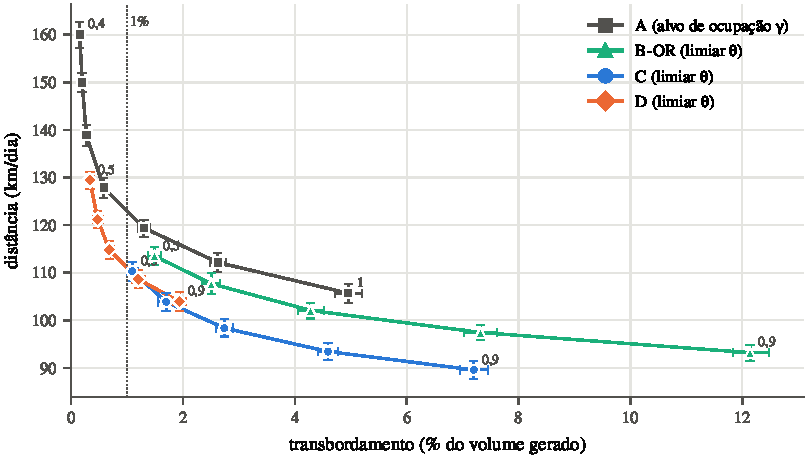
\includegraphics[width=\textwidth]{figures/fig_e2.pdf}
  \caption{E2 -- fronteiras distância $\times$ transbordamento ($N = 100$; 20 sementes por ponto; barras: IC 95\% nos dois eixos). Números junto aos pontos extremos: valor do parâmetro (ocupação-alvo $\gamma$ para A; limiar $\theta_{hi}$ para B-OR, C e D).}
  \label{fig:e2}
\end{figure}

A curva de A fica acima das demais em toda a faixa em que há sobreposição:
para manter o transbordamento em 1\% do volume gerado, A precisou, em média,
de \KmAtUmA{}~km/dia, contra \KmAtUmD{}~km/dia em D, uma redução de
\RelFrontUmDvsA\% (\NFrontUmDvsA{} sementes; $p_{\mathrm{Holm}}$
\PFrontUmDvsA). Com 2\% de transbordamento, a redução foi de
\RelFrontDoisCvsA\% para C e de \RelFrontDoisBORvsA\% para B-OR
(Tabela~\ref{tab:e2}). Onde as curvas de C e D se sobrepõem, elas ficam
próximas: com 2\%, D exigiu \RelFrontDoisDvsC\% de distância em relação a C
(\NFrontDoisDvsC{} sementes em que ambos alcançam o nível). B-OR, que não usa
contêineres opcionais, fica entre A e C.

\begin{table}[ht]
\centering
\caption{E2 -- distância necessária no mesmo nível de transbordamento (interpolação por semente; diferença em km/dia). Comparações com menos de 20 pares correspondem a sementes em que uma das políticas não alcança o nível dentro da faixa varrida.}
\label{tab:e2}
\scriptsize
\resizebox{\textwidth}{!}{\begin{tabular}{@{}llrcrrr@{}}
\toprule
Transb. & Comparação & Dif. média & IC 95\% & Dif. (\%) & $r_{rb}$ & $p$ (Holm) \\
\midrule
1,0\% & \polBOR{} $-$ \polA{} & $-$4,12 & [$-$5,51; $-$2,78] & $-$3,3 & $-$0,97 & $<$0,001 \\
1,0\% & \polC{} $-$ \polA{} & $-$10,84 & [$-$12,78; $-$9,01] & $-$8,8 & $-$1,00 & $<$0,001 \\
1,0\% & \polD{} $-$ \polA{} & $-$11,88 & [$-$13,55; $-$10,31] & $-$9,7 & $-$1,00 & $<$0,001 \\
1,0\% & \polD{} $-$ \polC{} & $-$1,03 & [$-$2,36; 0,31] & $-$0,9 & $-$0,33 & 0,202 \\
2,0\% & \polBOR{} $-$ \polA{} & $-$4,69 & [$-$5,66; $-$3,73] & $-$4,1 & $-$1,00 & $<$0,001 \\
2,0\% & \polC{} $-$ \polA{} & $-$13,07 & [$-$14,16; $-$12,00] & $-$11,3 & $-$1,00 & $<$0,001 \\
2,0\% & \polD{} $-$ \polA{} & $-$11,21 & [$-$12,02; $-$10,43] & $-$9,7 & $-$1,00 & $<$0,001 \\
2,0\% & \polD{} $-$ \polC{} & 1,86 & [1,03; 2,71] & 1,8 & 0,86 & $<$0,001 \\
\bottomrule
\end{tabular}
}
\end{table}

Essa análise muda a leitura do E1. A diferença entre C e D no E1 não indica
que a previsão seja necessária para obter ganhos; indica sobretudo que, com os
parâmetros padrão, C opera em um ponto de mais transbordamento da fronteira e
D em um ponto de menos. A vantagem robusta, observada em ambos, é a da seleção
orientada por dados sobre o calendário fixo: para o mesmo nível de serviço,
cerca de 10\% menos distância. A previsão serve, na prática, para alcançar
níveis baixos de transbordamento (abaixo de 1\%) que C só atinge com limiares
mais baixos e mais visitas. Esse valor, \RelFrontUmDvsA\%, é menor que os
ganhos médios relatados por estudos de simulação na meta-análise de
\cite{maciel2025impact} (cerca de 40\%) e próximo da média de implantações
reais (cerca de 12\%). Uma explicação plausível é que a linha de base aqui
é exigente: A tem frequências ajustadas contêiner a contêiner, com as taxas
médias verdadeiras, e rotas otimizadas pelo mesmo resolvedor.

\paragraph{Previsão.}
O preditor de taxa usado por D teve erro absoluto médio de \PredNCemD{} (em
fração do volume) para a ocupação 24~h à frente, contra \PersistNCemD{} da
persistência, em $N = 100$. Os erros foram calculados apenas para contêineres
sem coleta no intervalo e incluem o efeito do ruído de medição.

\subsection{Robustez a falhas de telemetria (E3)}\label{sec:e3}

O E3 perturba um fator por vez no cenário-base ($N = 100$). A
Tabela~\ref{tab:e3} mostra o transbordamento médio de cada política e a
disponibilidade de telemetria, e a Figura~\ref{fig:e3} mostra as mesmas médias
com seus intervalos. A política A não usa telemetria e serve de referência
fixa. A Tabela~\ref{tab:e3deg} compara cada condição com a base, dentro de
cada política.

\begin{table}[ht]
\centering
\caption{E3 -- transbordamento médio por condição e disponibilidade de telemetria (leituras válidas entregues/leituras programadas, na política C). Última coluna: distância de D. 30 sementes por célula; $N = 100$.}
\label{tab:e3}
\scriptsize
\resizebox{\textwidth}{!}{\begin{tabular}{@{}lrrrrrr@{}}
\toprule
 & Telemetria & \multicolumn{4}{c}{Transbordamento (\% do volume)} & km/dia \\
\cmidrule(lr){3-6}
Condição & disponível (\%) & \polA{} & \polBOR{} & \polC{} & \polD{} & \polD{} \\
\midrule
base & 97,2 & 1,28 & 5,77 & 3,61 & 0,92 & 112,2 \\
perda 5\% & 93,2 & 1,28 & 5,74 & 3,64 & 0,91 & 112,3 \\
perda 20\% & 78,5 & 1,28 & 5,82 & 3,61 & 0,88 & 113,1 \\
perda 50\% & 49,1 & 1,28 & 6,02 & 3,77 & 0,83 & 114,5 \\
interrupcao 48h & 84,8 & 1,28 & 6,36 & 4,06 & 0,89 & 113,2 \\
\bottomrule
\end{tabular}
}
\end{table}

\begin{figure}[ht]
  \centering
  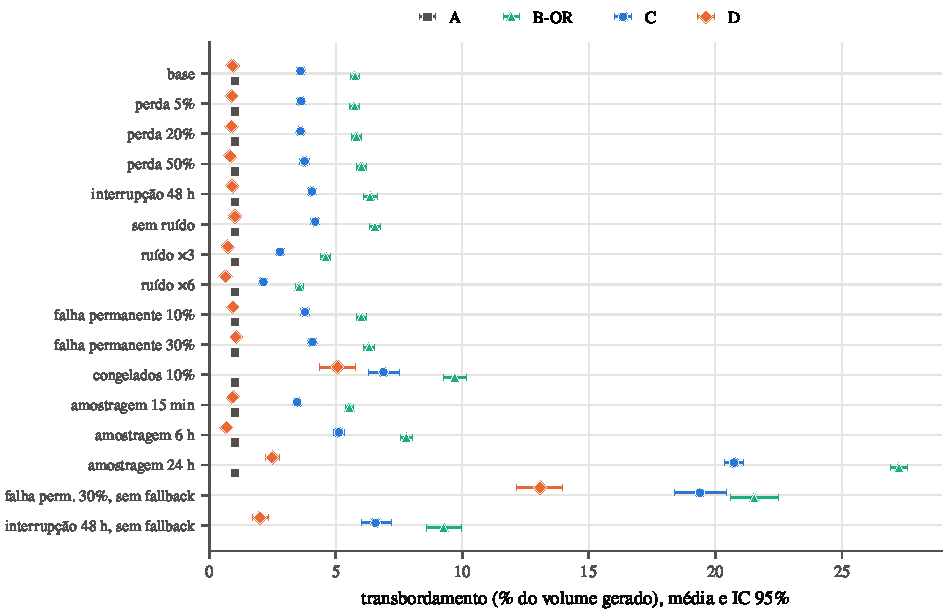
\includegraphics[width=\textwidth]{figures/fig_e3.pdf}
  \caption{E3 -- transbordamento por condição de telemetria (média e IC 95\%; 30 sementes; $N = 100$).}
  \label{fig:e3}
\end{figure}

\paragraph{Perda de mensagens e interrupções.}
Perdas independentes de 5\% e 20\% das mensagens não alteraram o
transbordamento de forma detectável em nenhuma política. Mesmo com 50\% de
perda, quando só metade das leituras chegou à plataforma, o efeito foi pequeno:
\DifETdegradacaoPerdaCZBORvsBOROv{} p.p. em B-OR ($p_{\mathrm{Holm}} =$
\PETdegradacaoPerdaCZBORvsBOROv), \DifETdegradacaoPerdaCZCvsCOv{} p.p. em C
(não significativo) e \DifETdegradacaoPerdaCZDvsDOv{} p.p. em D. Com uma
leitura por hora e decisões uma vez por dia, a plataforma tolera muitas
lacunas: basta que alguma leitura recente chegue antes do planejamento. As
interrupções regionais de 48~h, que deixam metade dos dispositivos sem
comunicação, tiveram efeito maior em B-OR
(+\DifETdegradacaoInterrupcaoQOHBORvsBOROv{} p.p.) e em C
(+\DifETdegradacaoInterrupcaoQOHCvsCOv{} p.p.; ambos $p_{\mathrm{Holm}}$
\PETdegradacaoInterrupcaoQOHCvsCOv), mas não em D
(\DifETdegradacaoInterrupcaoQOHDvsDOv{} p.p.; $p_{\mathrm{Holm}} =$
\PETdegradacaoInterrupcaoQOHDvsDOv).

\paragraph{Estimativa para dados desatualizados (H3b).}
O mecanismo de \emph{fallback}, que projeta a ocupação dos contêineres sem
dado recente pela taxa de longo prazo, foi decisivo. Com 30\% dos sensores em
falha permanente e o \emph{fallback} ativo, o transbordamento de C aumentou
\DifETdegradacaoFalhaPermTZCvsCOv{} p.p. em relação à base. Sem ele, isto é,
mantendo indefinidamente o último valor lido, o aumento foi de
\DifETdegradacaoFalhaPermTZSemFallbackCvsCOv{} p.p.; em D, de
\DifETdegradacaoFalhaPermTZDvsDOv{} p.p. com \emph{fallback} e
\DifETdegradacaoFalhaPermTZSemFallbackDvsDOv{} p.p. sem ele. Nas interrupções
de 48~h, desligar o \emph{fallback} elevou o aumento de C de
\DifETdegradacaoInterrupcaoQOHCvsCOv{} para
\DifETdegradacaoInterrupcaoQOHSemFallbackCvsCOv{} p.p. A hipótese H3b se
confirma. Um contêiner que para de reportar continua a encher, e uma
plataforma que trata o último valor lido como atual deixa de visitá-lo.

\paragraph{Falhas que a plataforma não detecta.}
Os sensores congelados (10\% dos dispositivos passam a repetir sempre a mesma
leitura, a partir de um instante sorteado) foram a perturbação mais grave
entre as de menor intensidade: +\DifETdegradacaoCongeladoUZBORvsBOROv{} p.p.
em B-OR, +\DifETdegradacaoCongeladoUZCvsCOv{} p.p. em C e
+\DifETdegradacaoCongeladoUZDvsDOv{} p.p. em D. O transbordamento de D
passou de valores próximos aos de A para cerca de cinco vezes o de A. Ao
contrário do sensor que se cala, o sensor congelado continua a enviar
mensagens válidas e recentes. O critério de desatualização não o identifica,
e o \emph{fallback} não é acionado. A ingestão implementada não verifica se
a ocupação permanece constante por tempo anormal. Essa verificação é simples
e deve preceder qualquer uso operacional (Seção~\ref{sec:limitacoes}).

\paragraph{Ruído e período de amostragem.}
O resultado contrário à hipótese H3a veio do ruído. Eliminar todo o erro de
medição \emph{aumentou} o transbordamento de B-OR, C e D
(+\DifETdegradacaoRuidoZBORvsBOROv, +\DifETdegradacaoRuidoZCvsCOv{} e
+\DifETdegradacaoRuidoZDvsDOv{} p.p.), e triplicar ou sextuplicar o ruído o
\emph{reduziu} (em C, \DifETdegradacaoRuidoTXCvsCOv{} e
\DifETdegradacaoRuidoSXCvsCOv{} p.p.), ao custo de mais distância
(Tabela~\ref{tab:e3}). O motivo está no modelo de medição
(Seção~\ref{sec:metodologia}). O termo de superfície irregular sempre encurta
a distância medida, porque o pulso reflete no pico da pilha. Por isso, ele
desloca a ocupação observada para cima, em média cerca de 0,8 vez o seu
desvio-padrão. Nas condições do E3, esse viés foi escalado junto com o ruído
simétrico e funcionou como margem de segurança: o contêiner parece mais cheio
do que está e é visitado antes. O E3, portanto, não separa o efeito do ruído
simétrico do efeito do viés sistemático, o que fica como limitação do
desenho. Em termos práticos, um limiar de 75\% sobre leituras enviesadas
para cima equivale a um limiar menor sobre a ocupação verdadeira, e a
calibração do sensor em campo altera o ponto de operação das políticas.

O período de amostragem separou as políticas. Com uma leitura a cada 6~h, o
transbordamento de C aumentou \DifETdegradacaoAmostraSHCvsCOv{} p.p.; com uma
a cada 24~h, \DifETdegradacaoAmostraDQHCvsCOv{} p.p., e o de B-OR,
\DifETdegradacaoAmostraDQHBORvsBOROv{} p.p. Em D, o aumento foi de
\DifETdegradacaoAmostraDQHDvsDOv{} p.p. com amostragem diária, e com 6~h o
transbordamento caiu (\DifETdegradacaoAmostraSHDvsDOv{} p.p.). As políticas
que decidem pelo valor observado dependem de dados frequentes, porque o valor
lido envelhece até o planejamento. A política que projeta a ocupação pela
taxa estimada compensa boa parte desse envelhecimento. Amostrar a cada 15
minutos, em vez de 1~h, não trouxe benefício relevante a nenhuma política.
Isso interessa ao projeto do dispositivo, porque cada leitura transmitida
consome energia.

\begin{table}[ht]
\centering
\caption{E3 -- variação do transbordamento em relação à base, dentro de cada política (p.p. do volume gerado; 30 pares; Holm na família E3/transbordamento).}
\label{tab:e3deg}
\scriptsize
\resizebox{\textwidth}{!}{\begin{tabular}{@{}llrcrrr@{}}
\toprule
Condição & Comparação & Dif. média & IC 95\% & Dif. (\%) & $r_{rb}$ & $p$ (Holm) \\
\midrule
perda 5\% & \polBOR{} (cond. $-$ base) & $-$0,02 & [$-$0,09; 0,04] & $-$0,4 & $-$0,11 & 1,000 \\
perda 20\% & \polBOR{} (cond. $-$ base) & 0,05 & [$-$0,02; 0,13] & 0,9 & 0,28 & 1,000 \\
perda 50\% & \polBOR{} (cond. $-$ base) & 0,25 & [0,15; 0,34] & 4,3 & 0,79 & 0,001 \\
interrupção 48 h & \polBOR{} (cond. $-$ base) & 0,59 & [0,41; 0,79] & 10,2 & 0,95 & $<$0,001 \\
sem ruído & \polBOR{} (cond. $-$ base) & 0,78 & [0,67; 0,89] & 13,6 & 1,00 & $<$0,001 \\
ruído $\times$3 & \polBOR{} (cond. $-$ base) & $-$1,16 & [$-$1,25; $-$1,07] & $-$20,1 & $-$1,00 & $<$0,001 \\
ruído $\times$6 & \polBOR{} (cond. $-$ base) & $-$2,21 & [$-$2,31; $-$2,10] & $-$38,2 & $-$1,00 & $<$0,001 \\
falha permanente 10\% & \polBOR{} (cond. $-$ base) & 0,24 & [0,14; 0,34] & 4,2 & 0,78 & 0,002 \\
falha permanente 30\% & \polBOR{} (cond. $-$ base) & 0,55 & [0,42; 0,68] & 9,5 & 0,97 & $<$0,001 \\
congelados 10\% & \polBOR{} (cond. $-$ base) & 3,94 & [3,49; 4,39] & 68,2 & 1,00 & $<$0,001 \\
amostragem 15 min & \polBOR{} (cond. $-$ base) & $-$0,23 & [$-$0,34; $-$0,11] & $-$3,9 & $-$0,71 & 0,008 \\
amostragem 6 h & \polBOR{} (cond. $-$ base) & 2,02 & [1,88; 2,15] & 35,0 & 1,00 & $<$0,001 \\
amostragem 24 h & \polBOR{} (cond. $-$ base) & 21,48 & [21,22; 21,73] & 372,4 & 1,00 & $<$0,001 \\
falha perm. 30\%, sem \emph{fallback} & \polBOR{} (cond. $-$ base) & 15,22 & [14,30; 16,18] & 240,8 & 1,00 & $<$0,001 \\
interrupção 48 h, sem \emph{fallback} & \polBOR{} (cond. $-$ base) & 2,91 & [2,37; 3,46] & 45,7 & 1,00 & $<$0,001 \\
perda 5\% & \polC{} (cond. $-$ base) & 0,03 & [$-$0,05; 0,12] & 0,8 & 0,05 & 1,000 \\
perda 20\% & \polC{} (cond. $-$ base) & 0,00 & [$-$0,08; 0,08] & $-$0,1 & $-$0,09 & 1,000 \\
perda 50\% & \polC{} (cond. $-$ base) & 0,16 & [0,04; 0,27] & 4,3 & 0,48 & 0,375 \\
interrupção 48 h & \polC{} (cond. $-$ base) & 0,45 & [0,31; 0,58] & 12,4 & 0,95 & $<$0,001 \\
sem ruído & \polC{} (cond. $-$ base) & 0,58 & [0,47; 0,70] & 16,1 & 0,99 & $<$0,001 \\
ruído $\times$3 & \polC{} (cond. $-$ base) & $-$0,81 & [$-$0,90; $-$0,72] & $-$22,5 & $-$1,00 & $<$0,001 \\
ruído $\times$6 & \polC{} (cond. $-$ base) & $-$1,47 & [$-$1,54; $-$1,39] & $-$40,7 & $-$1,00 & $<$0,001 \\
falha permanente 10\% & \polC{} (cond. $-$ base) & 0,18 & [0,07; 0,28] & 4,9 & 0,57 & 0,095 \\
falha permanente 30\% & \polC{} (cond. $-$ base) & 0,47 & [0,37; 0,57] & 13,0 & 0,99 & $<$0,001 \\
congelados 10\% & \polC{} (cond. $-$ base) & 3,28 & [2,69; 3,91] & 90,7 & 1,00 & $<$0,001 \\
amostragem 15 min & \polC{} (cond. $-$ base) & $-$0,13 & [$-$0,24; $-$0,02] & $-$3,6 & $-$0,45 & 0,469 \\
amostragem 6 h & \polC{} (cond. $-$ base) & 1,51 & [1,38; 1,64] & 41,9 & 1,00 & $<$0,001 \\
amostragem 24 h & \polC{} (cond. $-$ base) & 17,13 & [16,81; 17,43] & 474,5 & 1,00 & $<$0,001 \\
falha perm. 30\%, sem \emph{fallback} & \polC{} (cond. $-$ base) & 15,31 & [14,36; 16,30] & 375,3 & 1,00 & $<$0,001 \\
interrupção 48 h, sem \emph{fallback} & \polC{} (cond. $-$ base) & 2,51 & [2,02; 3,05] & 62,0 & 1,00 & $<$0,001 \\
perda 5\% & \polD{} (cond. $-$ base) & $-$0,02 & [$-$0,06; 0,03] & $-$1,8 & $-$0,10 & 1,000 \\
perda 20\% & \polD{} (cond. $-$ base) & $-$0,04 & [$-$0,09; 0,01] & $-$4,5 & $-$0,30 & 1,000 \\
perda 50\% & \polD{} (cond. $-$ base) & $-$0,09 & [$-$0,14; $-$0,04] & $-$9,7 & $-$0,66 & 0,024 \\
interrupção 48 h & \polD{} (cond. $-$ base) & $-$0,01 & [$-$0,06; 0,03] & $-$1,6 & $-$0,13 & 1,000 \\
sem ruído & \polD{} (cond. $-$ base) & 0,10 & [0,05; 0,14] & 10,3 & 0,70 & 0,010 \\
ruído $\times$3 & \polD{} (cond. $-$ base) & $-$0,18 & [$-$0,22; $-$0,14] & $-$19,7 & $-$0,96 & $<$0,001 \\
ruído $\times$6 & \polD{} (cond. $-$ base) & $-$0,28 & [$-$0,33; $-$0,23] & $-$30,1 & $-$0,99 & $<$0,001 \\
falha permanente 10\% & \polD{} (cond. $-$ base) & 0,02 & [$-$0,02; 0,06] & 2,3 & 0,14 & 1,000 \\
falha permanente 30\% & \polD{} (cond. $-$ base) & 0,13 & [0,07; 0,19] & 13,6 & 0,77 & 0,002 \\
congelados 10\% & \polD{} (cond. $-$ base) & 4,15 & [3,46; 4,88] & 448,7 & 1,00 & $<$0,001 \\
amostragem 15 min & \polD{} (cond. $-$ base) & 0,01 & [$-$0,04; 0,06] & 0,9 & 0,06 & 1,000 \\
amostragem 6 h & \polD{} (cond. $-$ base) & $-$0,24 & [$-$0,28; $-$0,19] & $-$25,5 & $-$1,00 & $<$0,001 \\
amostragem 24 h & \polD{} (cond. $-$ base) & 1,57 & [1,32; 1,84] & 169,5 & 1,00 & $<$0,001 \\
falha perm. 30\%, sem \emph{fallback} & \polD{} (cond. $-$ base) & 12,03 & [11,10; 12,90] & 1.145,3 & 1,00 & $<$0,001 \\
interrupção 48 h, sem \emph{fallback} & \polD{} (cond. $-$ base) & 1,10 & [0,82; 1,40] & 120,6 & 1,00 & $<$0,001 \\
\bottomrule
\end{tabular}
}
\end{table}

\subsection{Sensibilidade operacional (E4)}\label{sec:e4}

O E4 varia a demanda, a frota, o arranjo espacial e a velocidade. A
Figura~\ref{fig:e4} mostra, para cada condição, a diferença pareada de cada
política em relação a A, e as Tabelas~\ref{tab:e4km} e~\ref{tab:e4ov} trazem
os valores.

\begin{figure}[ht]
  \centering
  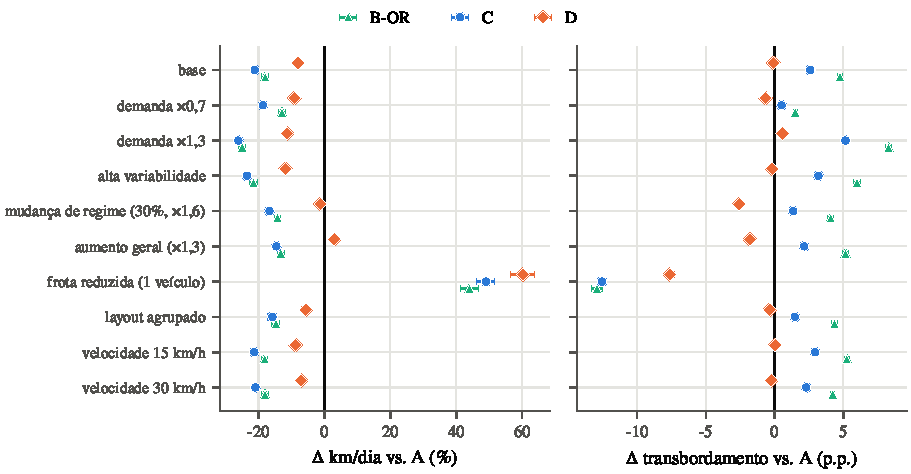
\includegraphics[width=\textwidth]{figures/fig_e4.pdf}
  \caption{E4 -- diferença pareada em relação a A por condição (média e IC 95\%; 30 sementes; $N = 100$). Esquerda: distância (\% de A); direita: transbordamento (pontos percentuais).}
  \label{fig:e4}
\end{figure}

\paragraph{Mudança na demanda (H4).}
A política A planeja o calendário com a taxa média verdadeira de cada
contêiner, mas não acompanha mudanças posteriores. Quando 30\% dos
contêineres passam a gerar 60\% a mais a partir do 14.º dia, o
transbordamento médio de A sobe de \OvNCemA\% para cerca de 4\%. O de D
sobe menos e fica \DifEQMudancaRegimeTZXUSDvsAOv{} p.p. em relação a A
($p_{\mathrm{Holm}}$ \PEQMudancaRegimeTZXUSDvsAOv), com distância
praticamente igual (\RelEQMudancaRegimeTZXUSDvsAKm\%). O mesmo padrão aparece
no aumento geral de 30\% da demanda (\DifEQSurtoGeralXUTDvsAOv{} p.p.), agora
com \RelEQSurtoGeralXUTDvsAKm\% de distância. C também se degrada menos que
A nessas condições, mas parte de um transbordamento maior e continua acima
dela. A hipótese H4 se confirma para mudanças de regime. É nelas que o
componente preditivo mostra seu valor mais claro. Quando a intensidade muda
desde o início e A a conhece (demanda $\times 0{,}7$ e $\times 1{,}3$), A
mantém cerca de 1\% de transbordamento. Ainda assim, com demanda baixa, D
reduziu ao mesmo tempo a distância (\RelEQDemandaZSeDvsAKm\%) e o
transbordamento (\DifEQDemandaZSeDvsAOv{} p.p.), e as reduções de distância
de C cresceram com a intensidade (\RelEQDemandaZSeCvsAKm\%,
\RelEQBaseCvsAKm\% e \RelEQDemandaUTCvsAKm\% para $\times 0{,}7$, base e
$\times 1{,}3$).

\paragraph{Frota insuficiente.}
Com um único veículo, a capacidade planejada (uma viagem de
26.000~L por turno, pela regra de execução do modelo) fica abaixo do
volume gerado por dia, e nenhuma política evita o transbordamento: A chegou a
31\%, e as demais ficaram entre 18\% e 24\% (Tabela~\ref{tab:e4ov}). Nessa
escassez, as políticas com telemetria transbordaram
\DifEQFrotaReduzidaCvsAOv{} p.p. (C) e \DifEQFrotaReduzidaDvsAOv{} p.p. (D)
em relação a A, porque priorizam os contêineres mais cheios. Em
contrapartida, percorreram mais (\RelEQFrotaReduzidaCvsAKm\% e
\RelEQFrotaReduzidaDvsAKm\%). Esse
resultado não indica que a telemetria substitua frota. Indica que, quando a
frota é insuficiente, os dados ajudam a decidir quem fica sem coleta.

\paragraph{Arranjo espacial e velocidade.}
Com contêineres agrupados em poucas áreas, todas as distâncias caem e D
reduziu a distância (\RelEQLayoutAgrupadoDvsAKm\%) e o transbordamento
(\DifEQLayoutAgrupadoDvsAOv{} p.p.) em relação a A. A velocidade do veículo
(15 ou 30~km/h) praticamente não alterou as diferenças relativas. No
cenário-base, a jornada de 8~h tem folga: em A, cada um dos dois veículos se
desloca cerca de 3~h por dia a 20~km/h.

\begin{table}[ht]
\centering
\caption{E4 -- comparações pareadas de km/dia por condição (alternativa $-$ referência; 30 pares; Holm na família E4/km).}
\label{tab:e4km}
\scriptsize
\resizebox{\textwidth}{!}{\begin{tabular}{@{}llrcrrr@{}}
\toprule
Condição & Comparação & Dif. média & IC 95\% & Dif. (\%) & $r_{rb}$ & $p$ (Holm) \\
\midrule
base & \polBOR{} $-$ \polA{} & $-$21,98 & [$-$23,19; $-$20,71] & $-$18,0 & $-$1,00 & $<$0,001 \\
base & \polC{} $-$ \polA{} & $-$25,81 & [$-$26,95; $-$24,61] & $-$21,2 & $-$1,00 & $<$0,001 \\
base & \polD{} $-$ \polA{} & $-$9,80 & [$-$10,97; $-$8,51] & $-$8,0 & $-$1,00 & $<$0,001 \\
base & \polD{} $-$ \polC{} & 16,01 & [15,28; 16,75] & 16,6 & 1,00 & $<$0,001 \\
demanda $\times$0,7 & \polBOR{} $-$ \polA{} & $-$12,69 & [$-$13,72; $-$11,66] & $-$12,9 & $-$1,00 & $<$0,001 \\
demanda $\times$0,7 & \polC{} $-$ \polA{} & $-$18,43 & [$-$19,49; $-$17,36] & $-$18,7 & $-$1,00 & $<$0,001 \\
demanda $\times$0,7 & \polD{} $-$ \polA{} & $-$8,98 & [$-$9,89; $-$8,03] & $-$9,1 & $-$1,00 & $<$0,001 \\
demanda $\times$0,7 & \polD{} $-$ \polC{} & 9,45 & [8,58; 10,24] & 11,8 & 1,00 & $<$0,001 \\
demanda $\times$1,3 & \polBOR{} $-$ \polA{} & $-$36,94 & [$-$38,49; $-$35,36] & $-$25,0 & $-$1,00 & $<$0,001 \\
demanda $\times$1,3 & \polC{} $-$ \polA{} & $-$38,63 & [$-$40,14; $-$37,10] & $-$26,1 & $-$1,00 & $<$0,001 \\
demanda $\times$1,3 & \polD{} $-$ \polA{} & $-$16,75 & [$-$18,07; $-$15,40] & $-$11,3 & $-$1,00 & $<$0,001 \\
demanda $\times$1,3 & \polD{} $-$ \polC{} & 21,89 & [21,09; 22,68] & 20,0 & 1,00 & $<$0,001 \\
alta variabilidade & \polBOR{} $-$ \polA{} & $-$27,56 & [$-$28,99; $-$26,11] & $-$21,5 & $-$1,00 & $<$0,001 \\
alta variabilidade & \polC{} $-$ \polA{} & $-$30,07 & [$-$31,46; $-$28,67] & $-$23,5 & $-$1,00 & $<$0,001 \\
alta variabilidade & \polD{} $-$ \polA{} & $-$15,08 & [$-$16,33; $-$13,94] & $-$11,8 & $-$1,00 & $<$0,001 \\
alta variabilidade & \polD{} $-$ \polC{} & 14,99 & [14,33; 15,64] & 15,3 & 1,00 & $<$0,001 \\
mudança de regime (30\%, $\times$1,6) & \polBOR{} $-$ \polA{} & $-$17,40 & [$-$18,65; $-$16,16] & $-$14,2 & $-$1,00 & $<$0,001 \\
mudança de regime (30\%, $\times$1,6) & \polC{} $-$ \polA{} & $-$20,38 & [$-$21,56; $-$19,18] & $-$16,7 & $-$1,00 & $<$0,001 \\
mudança de regime (30\%, $\times$1,6) & \polD{} $-$ \polA{} & $-$1,57 & [$-$2,82; $-$0,24] & $-$1,3 & $-$0,55 & 0,008 \\
mudança de regime (30\%, $\times$1,6) & \polD{} $-$ \polC{} & 18,82 & [18,07; 19,56] & 18,5 & 1,00 & $<$0,001 \\
aumento geral ($\times$1,3) & \polBOR{} $-$ \polA{} & $-$16,48 & [$-$17,87; $-$14,99] & $-$13,2 & $-$1,00 & $<$0,001 \\
aumento geral ($\times$1,3) & \polC{} $-$ \polA{} & $-$18,14 & [$-$19,38; $-$16,77] & $-$14,6 & $-$1,00 & $<$0,001 \\
aumento geral ($\times$1,3) & \polD{} $-$ \polA{} & 3,74 & [2,46; 5,25] & 3,0 & 0,94 & $<$0,001 \\
aumento geral ($\times$1,3) & \polD{} $-$ \polC{} & 21,88 & [21,05; 22,73] & 20,6 & 1,00 & $<$0,001 \\
frota reduzida (1 veículo) & \polBOR{} $-$ \polA{} & 23,60 & [22,19; 25,10] & 44,0 & 1,00 & $<$0,001 \\
frota reduzida (1 veículo) & \polC{} $-$ \polA{} & 26,30 & [24,81; 27,73] & 49,0 & 1,00 & $<$0,001 \\
frota reduzida (1 veículo) & \polD{} $-$ \polA{} & 32,29 & [30,24; 34,19] & 60,2 & 1,00 & $<$0,001 \\
frota reduzida (1 veículo) & \polD{} $-$ \polC{} & 5,99 & [4,36; 7,68] & 7,5 & 0,98 & $<$0,001 \\
layout agrupado & \polBOR{} $-$ \polA{} & $-$13,25 & [$-$14,53; $-$12,20] & $-$14,7 & $-$1,00 & $<$0,001 \\
layout agrupado & \polC{} $-$ \polA{} & $-$14,25 & [$-$15,49; $-$13,11] & $-$15,8 & $-$1,00 & $<$0,001 \\
layout agrupado & \polD{} $-$ \polA{} & $-$5,11 & [$-$6,25; $-$4,17] & $-$5,7 & $-$1,00 & $<$0,001 \\
layout agrupado & \polD{} $-$ \polC{} & 9,14 & [8,33; 9,95] & 12,0 & 1,00 & $<$0,001 \\
velocidade 15 km/h & \polBOR{} $-$ \polA{} & $-$22,12 & [$-$23,32; $-$20,89] & $-$18,2 & $-$1,00 & $<$0,001 \\
velocidade 15 km/h & \polC{} $-$ \polA{} & $-$25,93 & [$-$27,17; $-$24,72] & $-$21,3 & $-$1,00 & $<$0,001 \\
velocidade 15 km/h & \polD{} $-$ \polA{} & $-$10,68 & [$-$11,83; $-$9,48] & $-$8,8 & $-$1,00 & $<$0,001 \\
velocidade 15 km/h & \polD{} $-$ \polC{} & 15,25 & [14,69; 15,82] & 15,9 & 1,00 & $<$0,001 \\
velocidade 30 km/h & \polBOR{} $-$ \polA{} & $-$22,06 & [$-$23,26; $-$20,88] & $-$18,0 & $-$1,00 & $<$0,001 \\
velocidade 30 km/h & \polC{} $-$ \polA{} & $-$25,61 & [$-$26,88; $-$24,38] & $-$20,9 & $-$1,00 & $<$0,001 \\
velocidade 30 km/h & \polD{} $-$ \polA{} & $-$8,61 & [$-$9,71; $-$7,39] & $-$7,0 & $-$1,00 & $<$0,001 \\
velocidade 30 km/h & \polD{} $-$ \polC{} & 17,00 & [16,29; 17,68] & 17,6 & 1,00 & $<$0,001 \\
\bottomrule
\end{tabular}
}
\end{table}

\begin{table}[ht]
\centering
\caption{E4 -- comparações pareadas de transbordamento (p.p. do volume gerado; Holm na família E4/transbordamento).}
\label{tab:e4ov}
\scriptsize
\resizebox{\textwidth}{!}{\begin{tabular}{@{}llrcrrr@{}}
\toprule
Condição & Comparação & Dif. média & IC 95\% & Dif. (\%) & $r_{rb}$ & $p$ (Holm) \\
\midrule
base & \polBOR{} $-$ \polA{} & 4,76 & [4,59; 4,92] & 470,1 & 1,00 & $<$0,001 \\
base & \polC{} $-$ \polA{} & 2,60 & [2,47; 2,73] & 256,8 & 1,00 & $<$0,001 \\
base & \polD{} $-$ \polA{} & $-$0,09 & [$-$0,17; $-$0,01] & $-$8,7 & $-$0,40 & 0,115 \\
base & \polD{} $-$ \polC{} & $-$2,69 & [$-$2,80; $-$2,58] & $-$74,4 & $-$1,00 & $<$0,001 \\
demanda $\times$0,7 & \polBOR{} $-$ \polA{} & 1,50 & [1,34; 1,65] & 132,5 & 1,00 & $<$0,001 \\
demanda $\times$0,7 & \polC{} $-$ \polA{} & 0,51 & [0,35; 0,67] & 44,7 & 0,91 & $<$0,001 \\
demanda $\times$0,7 & \polD{} $-$ \polA{} & $-$0,65 & [$-$0,76; $-$0,55] & $-$57,8 & $-$1,00 & $<$0,001 \\
demanda $\times$0,7 & \polD{} $-$ \polC{} & $-$1,16 & [$-$1,28; $-$1,05] & $-$70,9 & $-$1,00 & $<$0,001 \\
demanda $\times$1,3 & \polBOR{} $-$ \polA{} & 8,30 & [8,09; 8,50] & 673,7 & 1,00 & $<$0,001 \\
demanda $\times$1,3 & \polC{} $-$ \polA{} & 5,16 & [4,97; 5,35] & 418,7 & 1,00 & $<$0,001 \\
demanda $\times$1,3 & \polD{} $-$ \polA{} & 0,58 & [0,49; 0,66] & 46,9 & 1,00 & $<$0,001 \\
demanda $\times$1,3 & \polD{} $-$ \polC{} & $-$4,58 & [$-$4,76; $-$4,40] & $-$71,7 & $-$1,00 & $<$0,001 \\
alta variabilidade & \polBOR{} $-$ \polA{} & 6,00 & [5,76; 6,24] & 151,6 & 1,00 & $<$0,001 \\
alta variabilidade & \polC{} $-$ \polA{} & 3,19 & [2,98; 3,39] & 80,7 & 1,00 & $<$0,001 \\
alta variabilidade & \polD{} $-$ \polA{} & $-$0,18 & [$-$0,32; $-$0,03] & $-$4,5 & $-$0,44 & 0,104 \\
alta variabilidade & \polD{} $-$ \polC{} & $-$3,37 & [$-$3,51; $-$3,22] & $-$47,1 & $-$1,00 & $<$0,001 \\
mudança de regime (30\%, $\times$1,6) & \polBOR{} $-$ \polA{} & 4,08 & [3,86; 4,29] & 97,0 & 1,00 & $<$0,001 \\
mudança de regime (30\%, $\times$1,6) & \polC{} $-$ \polA{} & 1,35 & [1,16; 1,54] & 32,2 & 1,00 & $<$0,001 \\
mudança de regime (30\%, $\times$1,6) & \polD{} $-$ \polA{} & $-$2,58 & [$-$2,72; $-$2,43] & $-$61,4 & $-$1,00 & $<$0,001 \\
mudança de regime (30\%, $\times$1,6) & \polD{} $-$ \polC{} & $-$3,93 & [$-$4,07; $-$3,79] & $-$70,8 & $-$1,00 & $<$0,001 \\
aumento geral ($\times$1,3) & \polBOR{} $-$ \polA{} & 5,16 & [4,94; 5,39] & 140,6 & 1,00 & $<$0,001 \\
aumento geral ($\times$1,3) & \polC{} $-$ \polA{} & 2,16 & [1,95; 2,38] & 58,7 & 1,00 & $<$0,001 \\
aumento geral ($\times$1,3) & \polD{} $-$ \polA{} & $-$1,80 & [$-$1,98; $-$1,61] & $-$48,9 & $-$1,00 & $<$0,001 \\
aumento geral ($\times$1,3) & \polD{} $-$ \polC{} & $-$3,95 & [$-$4,11; $-$3,80] & $-$67,8 & $-$1,00 & $<$0,001 \\
frota reduzida (1 veículo) & \polBOR{} $-$ \polA{} & $-$12,91 & [$-$13,28; $-$12,54] & $-$41,0 & $-$1,00 & $<$0,001 \\
frota reduzida (1 veículo) & \polC{} $-$ \polA{} & $-$12,56 & [$-$12,91; $-$12,20] & $-$39,9 & $-$1,00 & $<$0,001 \\
frota reduzida (1 veículo) & \polD{} $-$ \polA{} & $-$7,62 & [$-$7,96; $-$7,30] & $-$24,2 & $-$1,00 & $<$0,001 \\
frota reduzida (1 veículo) & \polD{} $-$ \polC{} & 4,94 & [4,77; 5,10] & 26,1 & 1,00 & $<$0,001 \\
layout agrupado & \polBOR{} $-$ \polA{} & 4,35 & [4,16; 4,55] & 437,6 & 1,00 & $<$0,001 \\
layout agrupado & \polC{} $-$ \polA{} & 1,48 & [1,36; 1,60] & 148,9 & 1,00 & $<$0,001 \\
layout agrupado & \polD{} $-$ \polA{} & $-$0,35 & [$-$0,42; $-$0,28] & $-$35,4 & $-$1,00 & $<$0,001 \\
layout agrupado & \polD{} $-$ \polC{} & $-$1,83 & [$-$1,95; $-$1,71] & $-$74,1 & $-$1,00 & $<$0,001 \\
velocidade 15 km/h & \polBOR{} $-$ \polA{} & 5,26 & [5,07; 5,46] & 497,4 & 1,00 & $<$0,001 \\
velocidade 15 km/h & \polC{} $-$ \polA{} & 2,95 & [2,80; 3,11] & 278,5 & 1,00 & $<$0,001 \\
velocidade 15 km/h & \polD{} $-$ \polA{} & 0,03 & [$-$0,06; 0,11] & 2,9 & 0,14 & 0,503 \\
velocidade 15 km/h & \polD{} $-$ \polC{} & $-$2,92 & [$-$3,06; $-$2,77] & $-$72,8 & $-$1,00 & $<$0,001 \\
velocidade 30 km/h & \polBOR{} $-$ \polA{} & 4,22 & [4,07; 4,38] & 422,8 & 1,00 & $<$0,001 \\
velocidade 30 km/h & \polC{} $-$ \polA{} & 2,30 & [2,15; 2,45] & 230,1 & 1,00 & $<$0,001 \\
velocidade 30 km/h & \polD{} $-$ \polA{} & $-$0,24 & [$-$0,31; $-$0,16] & $-$23,5 & $-$0,87 & $<$0,001 \\
velocidade 30 km/h & \polD{} $-$ \polC{} & $-$2,53 & [$-$2,66; $-$2,41] & $-$76,8 & $-$1,00 & $<$0,001 \\
\bottomrule
\end{tabular}
}
\end{table}

\subsection{Sensibilidade ao resolvedor (E5)}\label{sec:e5}

Com 500 contêineres, a descida gulosa do OR-Tools levou em média
\RefSolAT{}~s (A), \RefSolCT{}~s (C) e \RefSolDT{}~s (D) por planejamento
diário. A busca local guiada (GLS), interrompida após 5~s, encontrou rotas
mais curtas: a distância diária variou \RelSolAKm\% em A, \RelSolCKm\% em C e
\RelSolDKm\% em D ($p_{\mathrm{Holm}}$: \PSolAKm, \PSolCKm{} e \PSolDKm; 10
sementes). As diferenças são pequenas diante das diferenças entre políticas,
e a ordem se manteve com os dois resolvedores: com GLS, C percorreu
\AltSolCKm{}~km/dia, D \AltSolDKm{} e A \AltSolAKm. O transbordamento
praticamente não mudou (diferenças de \DifSolAOv, \DifSolCOv{} e
\DifSolDOv{}~p.p.). Como a melhoria do GLS foi um pouco maior em A, o uso da
descida gulosa nas rodadas principais tende a favorecer levemente as
políticas com telemetria, em menos de 1\% da distância de A. A escolha da
descida gulosa, motivada pelo determinismo, não altera as conclusões.

\subsection{Relação com a literatura}\label{sec:literatura}

As reduções de distância medidas aqui são menores que as frequentemente
relatadas por estudos de simulação. Com os parâmetros padrão, C percorreu
cerca de 21\% menos que A, mas transbordou mais. No mesmo nível de serviço, a
variação ficou entre \RelFrontUmCvsA\% e \RelFrontDoisCvsA\%. Duas escolhas de
desenho explicam boa parte da diferença. A primeira é que a linha de base usa
o mesmo resolvedor e frequências ajustadas por contêiner com taxas
verdadeiras. Muitos estudos comparam a coleta inteligente com uma rota fixa
pouco otimizada, o que mistura o efeito dos dados com o efeito da
roteirização. O E1 mostrou que essa mistura é grande: em $N = 100$ e $N = 500$, só trocar
o vizinho mais próximo pelo OR-Tools reduziu a distância de B em 17\% a 18\%. A
segunda escolha é medir o transbordamento junto com a distância. Uma política
que visita apenas contêineres acima de 75\% economiza distância, mas transfere
o custo para o serviço. \cite{brouwer2023comparison} descrevem o mesmo
compromisso entre número de coletas e número de transbordamentos. Os ganhos
modestos e a importância das hipóteses sobre a demanda também são coerentes
com a meta-análise de \cite{maciel2025impact}, em que os resultados de
implantações reais ficam bem abaixo dos de simulações.

\subsection{Implicações práticas}\label{sec:implicacoes}

Para um município que avalie sensores de nível, os resultados sugerem cinco
cuidados. Eles valem para o modelo estudado e precisam ser confirmados em
campo.
\begin{enumerate}
  \item Comparar com uma linha de base bem roteirizada. Parte do ganho da
        ``coleta inteligente'' pode ser obtida apenas com melhor roteirização
        da coleta atual.
  \item Fixar o nível de serviço antes de medir a economia. Reduções de
        distância obtidas com mais transbordamento não são ganhos de
        eficiência.
  \item Tratar dados ausentes explicitamente. A estimativa por taxa para
        contêineres sem dado recente foi a diferença entre degradação
        pequena e falha grave.
  \item Detectar sensores que continuam a reportar valores implausíveis
        (constantes, por exemplo). Esse é o modo de falha mais perigoso
        encontrado.
  \item Não superdimensionar a frequência de amostragem: uma leitura por hora
        foi suficiente, e a previsão compensou leituras ainda mais
        espaçadas.
\end{enumerate}
O valor dos dados aparece mais claramente quando a demanda muda e o calendário
fixo fica defasado, situação comum em áreas de crescimento urbano, eventos e
sazonalidade turística.

\subsection{Limitações}\label{sec:limitacoes}

Os resultados valem para o modelo e os parâmetros descritos. Os perfis de
geração, a heterogeneidade entre contêineres e os descartes volumosos são
hipóteses de cenário e não foram calibrados com medições de campo. As
posições dos contêineres e do depósito são hipotéticas, e os resultados não
descrevem o serviço real de Aracaju. O veículo percorre a malha a velocidade
constante, sem trânsito, e cada veículo faz uma rota planejada por turno, com
desvios ao depósito apenas quando a carga excede a capacidade. Por isso, o
cenário de frota reduzida mede sobretudo a restrição de capacidade. O
transbordamento é modelado como volume recusado, sem efeitos sobre os
contêineres vizinhos ou sobre o comportamento da população. O E3 não separa o
ruído simétrico do viés da superfície irregular, e os fatores do E3 e do E4
foram variados um de cada vez, sem estimar interações. O resolvedor é
heurístico, e a qualidade das rotas pode variar com o tamanho da instância
(Seção~\ref{sec:e5}). A plataforma não detecta sensores congelados. O
firmware foi compilado, mas não executado em hardware, e a integração MQTT
foi verificada com dispositivos virtuais em \emph{broker} local, não em rede
celular ou Wi-Fi urbana. Por fim, a política A recebe as taxas médias
verdadeiras, um planejador que nenhum município possui. Uma linha de base
estimada com histórico real tenderia a ser pior, e as diferenças em relação a
ela seriam maiores. Esse efeito não foi quantificado.

